\chapter[Metodología]{Metodología propuesta}{Metodología Propuesta}\label{Metodologia}
\crefname{section}{sección}{}
\crefname{table}{tabla}{}
\crefformat{equation}{#2ecuación #1#3}

\noindent
\rule{0.49\textwidth}{0.75pt} $_{\bigcirc}$ \rule{0.49\textwidth}{0.75pt}\\

La metodología se basa en la recolección de datos, el pre-procesamiento de los mismos, en fases de entrenamiento para los distintos modelos usados y su respectiva validación con sus indicadores de error y eficiencia.\\
Para mejorar la calidad de la toma de decisiones de inversión se agregó un análisis de métricas antes de la fase de entrenamiento para saber cuáles son las características de la blockchain que más variabilidad agregan al precio. Por último se hizo una inspección a los datos usando análisis topológico para poder predecir posibles tiempos de crisis.\\
Los resultados de esta metodología es un posible precio en un intervalo de tiempo futuro, una recomendación de inversión y una posible advertencia de un crac en la serie de tiempo financiera.\\
%Al final de este flujo de trabajo se toma una decisión para invertir 

\noindent
\rule{0.49\textwidth}{0.75pt} $_{\bigcirc}$ \rule{0.49\textwidth}{0.75pt}\\
\clearpage

\section{Metodología}
La metodología general del trabajo se muestra en la \cref{fig4}. Esta se divide en el pre-procesamiento de los datos, entrenamiento de modelos, análisis de métricas, análisis topológico de datos y validación.
El procedimiento propuesta se divide en cuatro apartados: La predicción del precio utilizando series de tiempo del bitcoin en dólares, el análisis de las métricas de la blockchain, la clasificación de las alzas y bajas del precio y el análisis topológico de datos.
 
En la predicción del precio se darán a conocer rendimientos futuros utilizando un conjunto de datos de prueba sobre el cual se realizará la predicción usando modelos estadísticos y de machine learning. Para el análisis de métricas de la blockchain se encontrarán las variables que más influyen en el precio del bitcoin utilizando análisis de regresión, análisis de componentes principales y clustering jerárquico, por otra parte la clasificación para toma de decisiones de inversión a mediano y largo plazo convertirá la serie de tiempo en imágenes y las clasificará en comprar, vender o incertidumbre utilizando redes neuronales convolucionales, por último, el análisis topológico de datos analizará posibles cracs en el precio utilizando la norma topológica $C^1$ y K-means. 
\vspace{-0.59cm}
\subsection{Datos y pre-procesamiento}
Los datos del precio del bitcoin están disponibles en linea de forma gratuita. Los datos para este estudio fueron recolectados de tres fuentes distintas, Yahoo Finance \parencite{YahooFinanceStock}, Kraken \parencite{BitcoinCryptocurrencyExchange} e Investing \parencite{InvestingComStock}. Para la descarga de estos datos se usó la librería \emph{quandl} en Python para descargarlos de forma automática en formato OHLCV (Open-High-Low-Close-Volume). Este formato consiste en un marco de datos indizados por la fecha y con columnas el precio de apertura, el precio más bajo del día, el más alto y el precio de cierre. El intervalo de los datos es considerado desde el 2 de febrero del 2012 hasta el 14 de abril de 2022.
Las tres fuentes de datos mostraban diferencias al compararlas, no todas estaban en formato OHLCV y habían gaps entre los precios. Para solucionar lo anterior se creó la función \emph{merge\_dfs\_on\_column} en Python, que tiene por entrada una lista de dataframes con columnas en común, una lista con los nombres de exchanges usados asociados a los dataframes y la columna en común sobre la cual se trabajará. Esta función devuelve un dataframe que combina las columnas en común especificadas. Las columnas de dataframe obtenido anteriormente son sumadas y dividas entre el número de columnas, creándose así una única columna con la media.

\begin{landscape}
	\begin{figure}
		\centering
		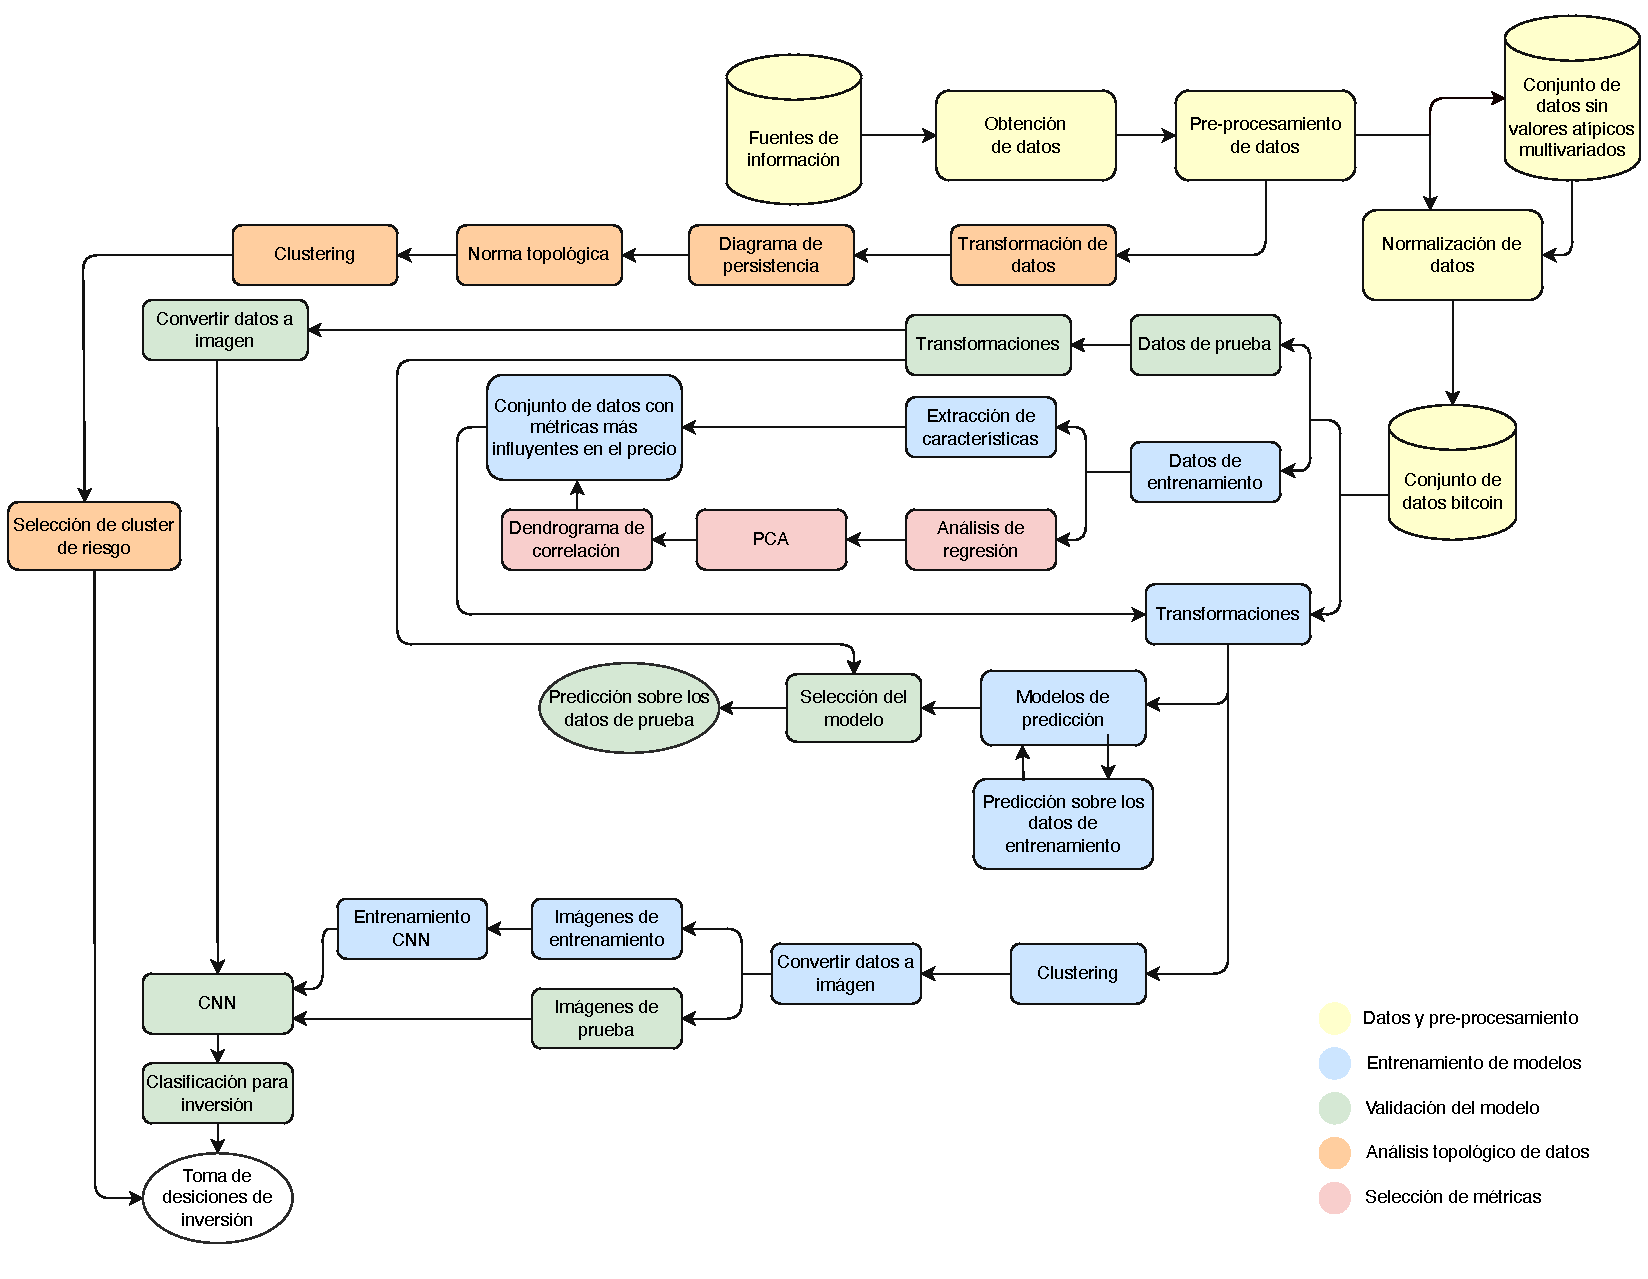
\includegraphics[scale=0.7]{Chapter3/Meto-3.pdf}
		\caption{Metodología general propuesta para la toma de decisiones de inversión.}
		\label{fig4}
	\end{figure}
\end{landscape}

Al final se crea un conjunto de datos usando como columnas las medias obtenidas utilizando la función antes especificada. 
%Ya que algunos exchanges no registran los precios con precisión o no trabajan en días festivos o fines de semana, entonces se eliminan estas fechas al dataframe creado con la media de los precios y se inputan los datos faltantes utilizando interpolación splines cúbico en ambas direcciones.\\
Los datos para realizar el análisis de métricas fueron recolectados utilizando la API de la comunidad de Coin Metrics \parencite{APIBasics}. Las métricas obtenidas en formato CSV fueron un total de 140 y se muestran en la \cref{tab:Table13} y \cref{tab:Table14}. Se consideró un intervalo de los datos desde el 2 de febrero del 2012 hasta el 14 de abril de 2022 donde se utilizó interpolación de splines de orden tres para igualmente rellenar datos faltantes.

Se eliminaron los valores atípicos multivariados del conjunto de datos de métricas utilizando la distancia de  Mahalanovis definida como
\[ D_M(x) = \sqrt{(x-\mu)\textbf{S}^{-1}(x-\mu)}, \]
donde $x = (x_1,x_2,x_3,...,x_N)^T$ es una observación, $\mu = (\mu_1,\mu_2,\mu_3,...,\mu_N)^T$ es la media y $\textbf{S}$ es la matriz de covarianza. Un valor se considera atípico si la distancia del dato (la métrica en este caso) encontrada es mayor que dos veces la media de las distancias.

Se escalaron los datos de las métricas como del precio al intervalo [0,1] con la formula $(x-min(x))/(max(x)-min(x))$ del método MinMax para un mejor funcionamiento de los algoritmos de aprendizaje máquina. 	 

\subsection{Entrenamiento de modelos}

Las bases de datos creadas se dividieron en un 80\% para los datos de entrenamiento y en un 20\% para los datos de prueba. Para los datos de predicción el conjunto de entrenamiento contiene 2980 elementos. Para el conjunto de entrenamiento de métricas de la blockchain se utilizó la función \emph{train\_test\_split} de la librería sklearn en Python conteniendo 3725 datos. Por último, después de las transformaciones correspondientes el conjunto de entrenamiento para clasificación y toma de decisiones de inversión resultó en 1040 imágenes.

\subparagraph{Predicción del precio:}
\label{met:prediccion}
Para la extracción de características de los modelos de aprendizaje máquina se usó el método de correlación \parencite{tandonBitcoinPriceForecasting2019}, donde se realizó la estimación del coeficiente de correlación de Pearson para examinar la fuerza y la dirección de la relación lineal entre las variables de la base de datos, en este caso, apertura, precio máximo, mínimo y cierre. Se determinó que todas las características están fuertemente relacionadas entre sí y fueron utilizadas como variables explicativas en los modelos no univariados (SVM, RF, RTS). A las características extraídas se les agregó las métricas de la blockchain que más influyeron en la variabilidad del precio como se detalla en la \cref{ssec:metrics}.    
Para las redes LSTM se utilizó únicamente el precio de cierre con retraso de un día para su ajuste.

Antes de aplicar los modelos a los datos de entrenamiento se realizaron distintas transformaciones como BoxCox [\ref{eqn:9}], $\log$ [\ref{eqn:10}], diff [\ref{eqn:11}] y diff($\log$) [\ref{eqn:12}] que se explican en la \cref{transformacionesmatematicas}. Para la transformación BoxCox el parámetro $\lambda$ se estimó con la función BoxCox.lambda() de R para encontrar el parámetro que mejor estabiliza la varianza, en el caso de la transformación $\log$ se uso la base natural $e$.

Se ajustaron los precios del bitcoin usando diferentes modelos estadísticos y de machine learning basados en los métodos Naive [\ref{eqn:1}], SES [\ref{eqn:2}], Holt [\ref{eqn:3}], ETS \footnotemark , ARIMA [\ref{eqn:4}], RTS [\ref{eqn:5}], SVM [\ref{eqn:6}], RF [\ref{eqn:7}], y LSTM [\ref{eqn:8}] que se explican en la \cref{modelosestadisticos} y la \cref{modelosmachinelearning}.

Para los métodos Naive, SES, Holt, ETS y ARIMA se usaron las funciones estándar de R del paquete \emph{fpp2}, únicamente cambiando la entrada de los datos de entrenamiento por la respectiva transformación, por otro lado, para el método RTS, SVM y RF se realizaron las inferencias sobre las características dichas anteriormente, manteniendo los hiperparámetros por defecto. La configuración usada para el modelos LSTM es la mostrada en la \cref{tab:Table10}.

%Tabla hiperparámetros LSTM
\begin{table}[!h]
	\centering
	\begin{tabular}{p{4cm} p{4cm}  }
		\toprule
		\textbf{Hiperparámetro} & \textbf{Configuración}\\
		\midrule
		Optimizer & Adam\\
		Hidden layers & 2 (2,1)\\
		Learning rate & 0.02\\
		Epochs & 100\\
		Batch size & 1\\
		Activation & tanh\\
		Loss function & MSE\\
		\bottomrule
		\hline
	\end{tabular}
	\caption{Configuración de los hiperparámetros LSTM.}
	\label{tab:Table10}
\end{table}

%Tabla transformaciones
\begin{table}[h]
	\centering
	\begin{tabular}{m{4cm} m{8cm}}
		\toprule
		\textbf{Transformación} & \textbf{\hspace{4cm}Fórmula}\\
		\midrule
		BoxCox			& 
		
		\begin{equation}
			\label{eqn:9}
			y_{t}(\lambda)= \left\{ \begin{array}{lcc}
				
				\frac{y_{t}^{\lambda} - 1}{\lambda} &   si  & \lambda \neq 0 \\
				\log{y_{t}} &  si & \lambda = 0 \\
				
			\end{array}
			\right.
		\end{equation}  
		\\ 
		log			&
		\begin{equation}
			\label{eqn:10}
			y_{t} = \log{y_{t}}
		\end{equation} \\
		\emph{diff} 			&
		\begin{equation}
			\label{eqn:11}
			\nabla y_{t} = y_{t} - y_{t-1}
		\end{equation}
		\\
		\emph{diff}(log)		& 
		\begin{equation}
			\label{eqn:12}
			\nabla y_{t} = \log{y_{t}} - \log{y_{t-1}}
		\end{equation}\\
		\bottomrule
		\hline
	\end{tabular}
	\caption{Transformaciones utilizadas en los modelos de entrenamiento.}
	\label{tab:Table9}
\end{table}

\footnotetext[1]{Encuentra el modelo que minimiza mejor el AIC (Akaike’s Information Criterion) o BIC (Schwarz’s Bayesian Information Criterion) usando SES de primer, segundo o tercer orden.}

%Tabla modelos utilizados
\begin{table*}
	\centering
	\begin{adjustbox}{width=0.95\textwidth}
	\begin{tabular} {m{2cm} m{9cm} m{7cm}}
		\toprule
		\textbf{Modelo} & \textbf{\hspace{3cm}Notación} & \textbf{Parámetros}\\
		\midrule
		Naive&\begin{equation}\label{eqn:1}\hat{y}_{t+h \mid t} = y_{t}\end{equation}	  
		&\\
		SES&	
		\begin{align}
			\label{eqn:2}
			\begin{split}
				\hat{y}_{t+h\mid t} = l_{t}
				\\
				l_{t} = \alpha y_{t}+(1-\alpha)l_{t-1}
			\end{split}
		\end{align}
		& $0 \leq \alpha \leq 1$\\
		Holt 	&	
		\begin{align}
			\label{eqn:3}
			\begin{split}
				\hat{y}_{t+h\mid t} = l_{t}+hb_{t}
				\\
				l_{t} = \alpha y_{t}+(1-\alpha)(l_{t-1}+b_{t-1})
				\\
				b_{t} = \beta(l_{t}-l_{t-1})+(1-\beta)b_{t-1}
			\end{split}
		\end{align}
		& $0 \leq \alpha \leq 1$
		\newline $0 \leq \beta \leq 1$
		\\
		ETS\footnotemark	& &
		\\
		ARIMA 	&	
		\begin{align}
			\label{eqn:4}
			\begin{split}
				\nabla y_{t} = c + \phi \nabla_{1} y_{t-1}+...+\phi \nabla_{p} y_{t-p}\\
				+\theta_{1}\epsilon_{t-1}+...+\theta_{q}\epsilon_{t-q}+\epsilon_{t}
			\end{split}
		\end{align}
		& 
		$p$: orden de parte autorregresiva\newline
		$d$: grado de las diferencias\newline
		$q$: orden de promedios móviles\newline
		$\phi ,\theta\in R$\newline
		\\
		RTS 		&	
		\begin{align}
			\label{eqn:5}
			\begin{split}
				y_{t} = \beta_{0}+\beta_{1}x_{1,t}+...+\beta_{k}x_{k,t}+\epsilon_{t}
			\end{split}
		\end{align}
		&
		$\beta_i\in R, i\in\{1,...,k\}$\newline
		\\
		SVM 		&	
		\begin{align}
			\label{eqn:6}
			\begin{split}
				\textrm{min} \frac{1}{2}\|w\|^{2}+\nu\sum_{i=1}^{m}\xi_{i}\\
				\textrm{s.a}\hspace{0.1cm} y_{i}(wx_{i}-b)\geq  1-\xi_{i},\hspace{0.1cm} \xi\geq 0
			\end{split}
		\end{align}
		&
		$w\in R^{n}$\newline
		$b\in R$\newline 
		$\nu$ parámetro de regularización \newline
		$\xi_{i}$ variables de holgura
		\\
		RF 		&	
		\begin{align}
			\label{eqn:8}
			\begin{split}
				g_{c}(x)=\frac{1}{t}\sum_{j=1}^{t}\hat{P}(c\mid v_{j}(x))\\
				P(c\mid v_{j}(x)) = \frac{P(c, v_{j}(x))}{\sum_{l=1}^{n}P(c_{l},v_{j}(x))}	
			\end{split}
		\end{align}
		&
		$t$: número de árboles creados en un subespacio aleatorio\newline
		$c$: clase 1,2,...,n\newline
		$v_{j}(x)$: nodo terminal del punto $x$ en el árbol $T_{j}$ ($j = 1,2,...,t$)
		\\
		LSTM 	&	
		\begin{align}
			\label{eqn:7}
			\begin{split}
				x = \left[ \begin{array}{c} x_{t} \\ h_{t-1} \end{array} \right]\\
				f_{t} = \delta(W_{f}X+b_{f})\\
				i_{t} = \delta(W_{i}X+b_{i})\\
				o_{t} = \delta(W_{o}X+b_{o})\\
				\tilde{C}_{t} = \tanh (W_{c}[h_{t-1},x_{t}]+b_{c})\\
				C_{t} = f_{t} \cdot C_{t-1}+i_{t} \cdot \tilde{C}_{t}\\
				h_{t} = o_{t}\cdot \tanh(C_{t})
			\end{split}
		\end{align}
		& 
		$x_{t}$: entrada al tiempo $t$ \newline
		$h_{t}$: estado oculto al tiempo $t$	\newline
		$W_{f},W_{i},W_{o},W_{c}$: matrices de peso\newline
		$b_{f},b_{i},b_{o},b_{c}$: parámetros de entrenamiento\newline
		$\delta$: función de activación
		\\
		\bottomrule
	\end{tabular}
	\end{adjustbox}
	\caption{Descripción de modelos usados en la comparación.}
	\label{tab:Table8}
\end{table*}

\footnotetext[2]{Generalización del modelo SES que toma en cuenta el error, la tendencia y la estacionalidad.}

\subparagraph{Clasificación para toma de decisiones de inversión:} Después del pre-procesamiento de los datos se aplica una transformación logarítmica al precio de cierre en dólares para estabilizar la varianza. El objetivo de esta transformación es tratar de identificar una tendencia monótona dada por
\begin{equation}
	\textrm{TSF}(x) = \log(x).
	\label{eqn:ajuste}
\end{equation}
En este estudio nos referimos al ajuste de la \cref{eqn:ajuste} como la \textbf{característica estadística tradicional} (TSF)\parencite{pinedo-sanchezVibrationAnalysisBearings2020}.\\

La entropía de Shannon es fundamental en la teoría de la información y también es conocida por medir la incertidumbre. La ecuación original es
\[ H(x) = -\sum_{i=1}^{n}p(x_i)\log{p(x_i)}, \]
donde $x$ es una variable aleatoria discreta con posibles salidas $x_1,x_2,x_3,...,x_n$. Entonces como en el articulo de Ben Ali et al. \parencite*{benaliNewEnhancedFeature2014} se utilizó una modificación de esta ecuación que tiene la forma
\[ H(x) = \frac{1}{n} \sum_{i=1}^{n}-\textrm{TSF}(x_i)\log_2{\textrm{TSF}(x_i)}, \]
aquí $n$ es el tamaño de la ventana deslizante. Esta última ecuación permite destacar las características obtenidas de la TSF. De este modo se puede elegir el TSF junto con la entropía de Shannon para observar un aumento o disminución bien definidos de los datos a lo largo del tiempo.

Se crea un plano que tiene por eje $x$ la entropía calculada y por eje $y$ la norma topológica $C^1$, que se obtiene como se detalla en \cref{met_tda}.


El siguiente paso es agrupar los datos del plano anterior después de las transformaciones correspondientes para así tener las etiquetas que clasifiquen los precios del bitcoin. Se utilizó el algoritmo K-means para agrupar los datos con características similares. Este algoritmo consiste en minimizar la suma de las distancias euclidianas de cada uno de los puntos con respecto al centroide del cluster. Se utilizó con $k=10$ para una mayor precisión a la hora de escoger los grupos para la toma de decisiones de inversión.

Los grupos creados se trasladan a los datos del precio originales desde el cual, manualmente se escogen los clusters de vender, comprar o incertidumbre.

El proceso para convertir los datos a imágenes con datos originales $R$ y $N$ puntos de muestreo se observan en la \cref{fig: met5}.  Si las imágenes a generar son de una resolución de $M \times M$, entonces el primer paso es tomar una sub-muestra $L$ de tamaño $M^2$ de los datos originales $R$, esto es, la i-ésima muestra esta dada por la expresión 

\[ L_i = \{R(i\cdot s+1),R(i\cdot s+2),R(i\cdot s+3),...,R(i\cdot s+M^2)\}, \]

donde $s\in \mathbb{Z}^+$ es el paso entre muestras y el índice $i = \{1,2,3,...,  \lfloor\frac{N}{s}\rfloor\}$, con $\lfloor \cdot \rfloor$ la función piso. Cada punto de la sub-muestra $L$ llena una matriz de $M\times M$ de izquierda a derecha y de arriba a abajo. Cada punto es normalizado de $0$ a $255$ y representa el valor del píxel en una escala de grises. Para la i-ésima imagen $P(x,y)$ el proceso se define como sigue

\[ P_i(x,y) =  \textrm{round}\left(\frac{L_i\{(x-1)\cdot M+y\}-\min(L_i)}{\max(L_i)-\min(L_i)}\cdot 255\right).\]
Para el propósito de este estudio se ha escogido una resolución de $32\times 32$ píxeles con un paso $s = 32$.    

La configuración de la arquitectura utilizada esta basada en AlexNet y se muestra en la \cref{tab:Table11}. Esta mostró ser la optima en un estudio del desgaste de baleros con una precisión por arriba del $98.64\%$, mostrando que usar una arquitectura basada en AlexNet sobre imágenes generadas sobre series de tiempo da buenos resultados \parencite{pinedo-sanchezVibrationAnalysisBearings2020}. 

%Arquitectura CNN
\begin{table}[h]
	\centering
	\begin{tabular}{m{1cm} m{3cm}  }
		\toprule
		\textbf{Capa} & \textbf{Característica}\\
		\midrule
		1 & Conv($5\times 5 \times 96$)\\
		2 & Maxpool($2\times 2$)\\
		3 & Conv($3\times 3 \times 256$)\\
		4 & Maxpool($2\times 2$)\\
		5 & Conv($3\times 3 \times 384$)\\
		6 & Maxpool($2\times 2$)\\
		7 & Conv($3\times 3 \times 384$)\\
		8 & Conv($3\times 3 \times 256$)\\
		9 & Maxpool($2\times 2$)\\
		10 & FC ($n$)\\
		11 & FC ($n$)\\
		12 & FC ($x$)\\
		\bottomrule
		\hline
	\end{tabular}
	\caption{Configuración de la arquitectura propuesta.}
	\label{tab:Table11}
\end{table}
\begin{figure}[h!]
	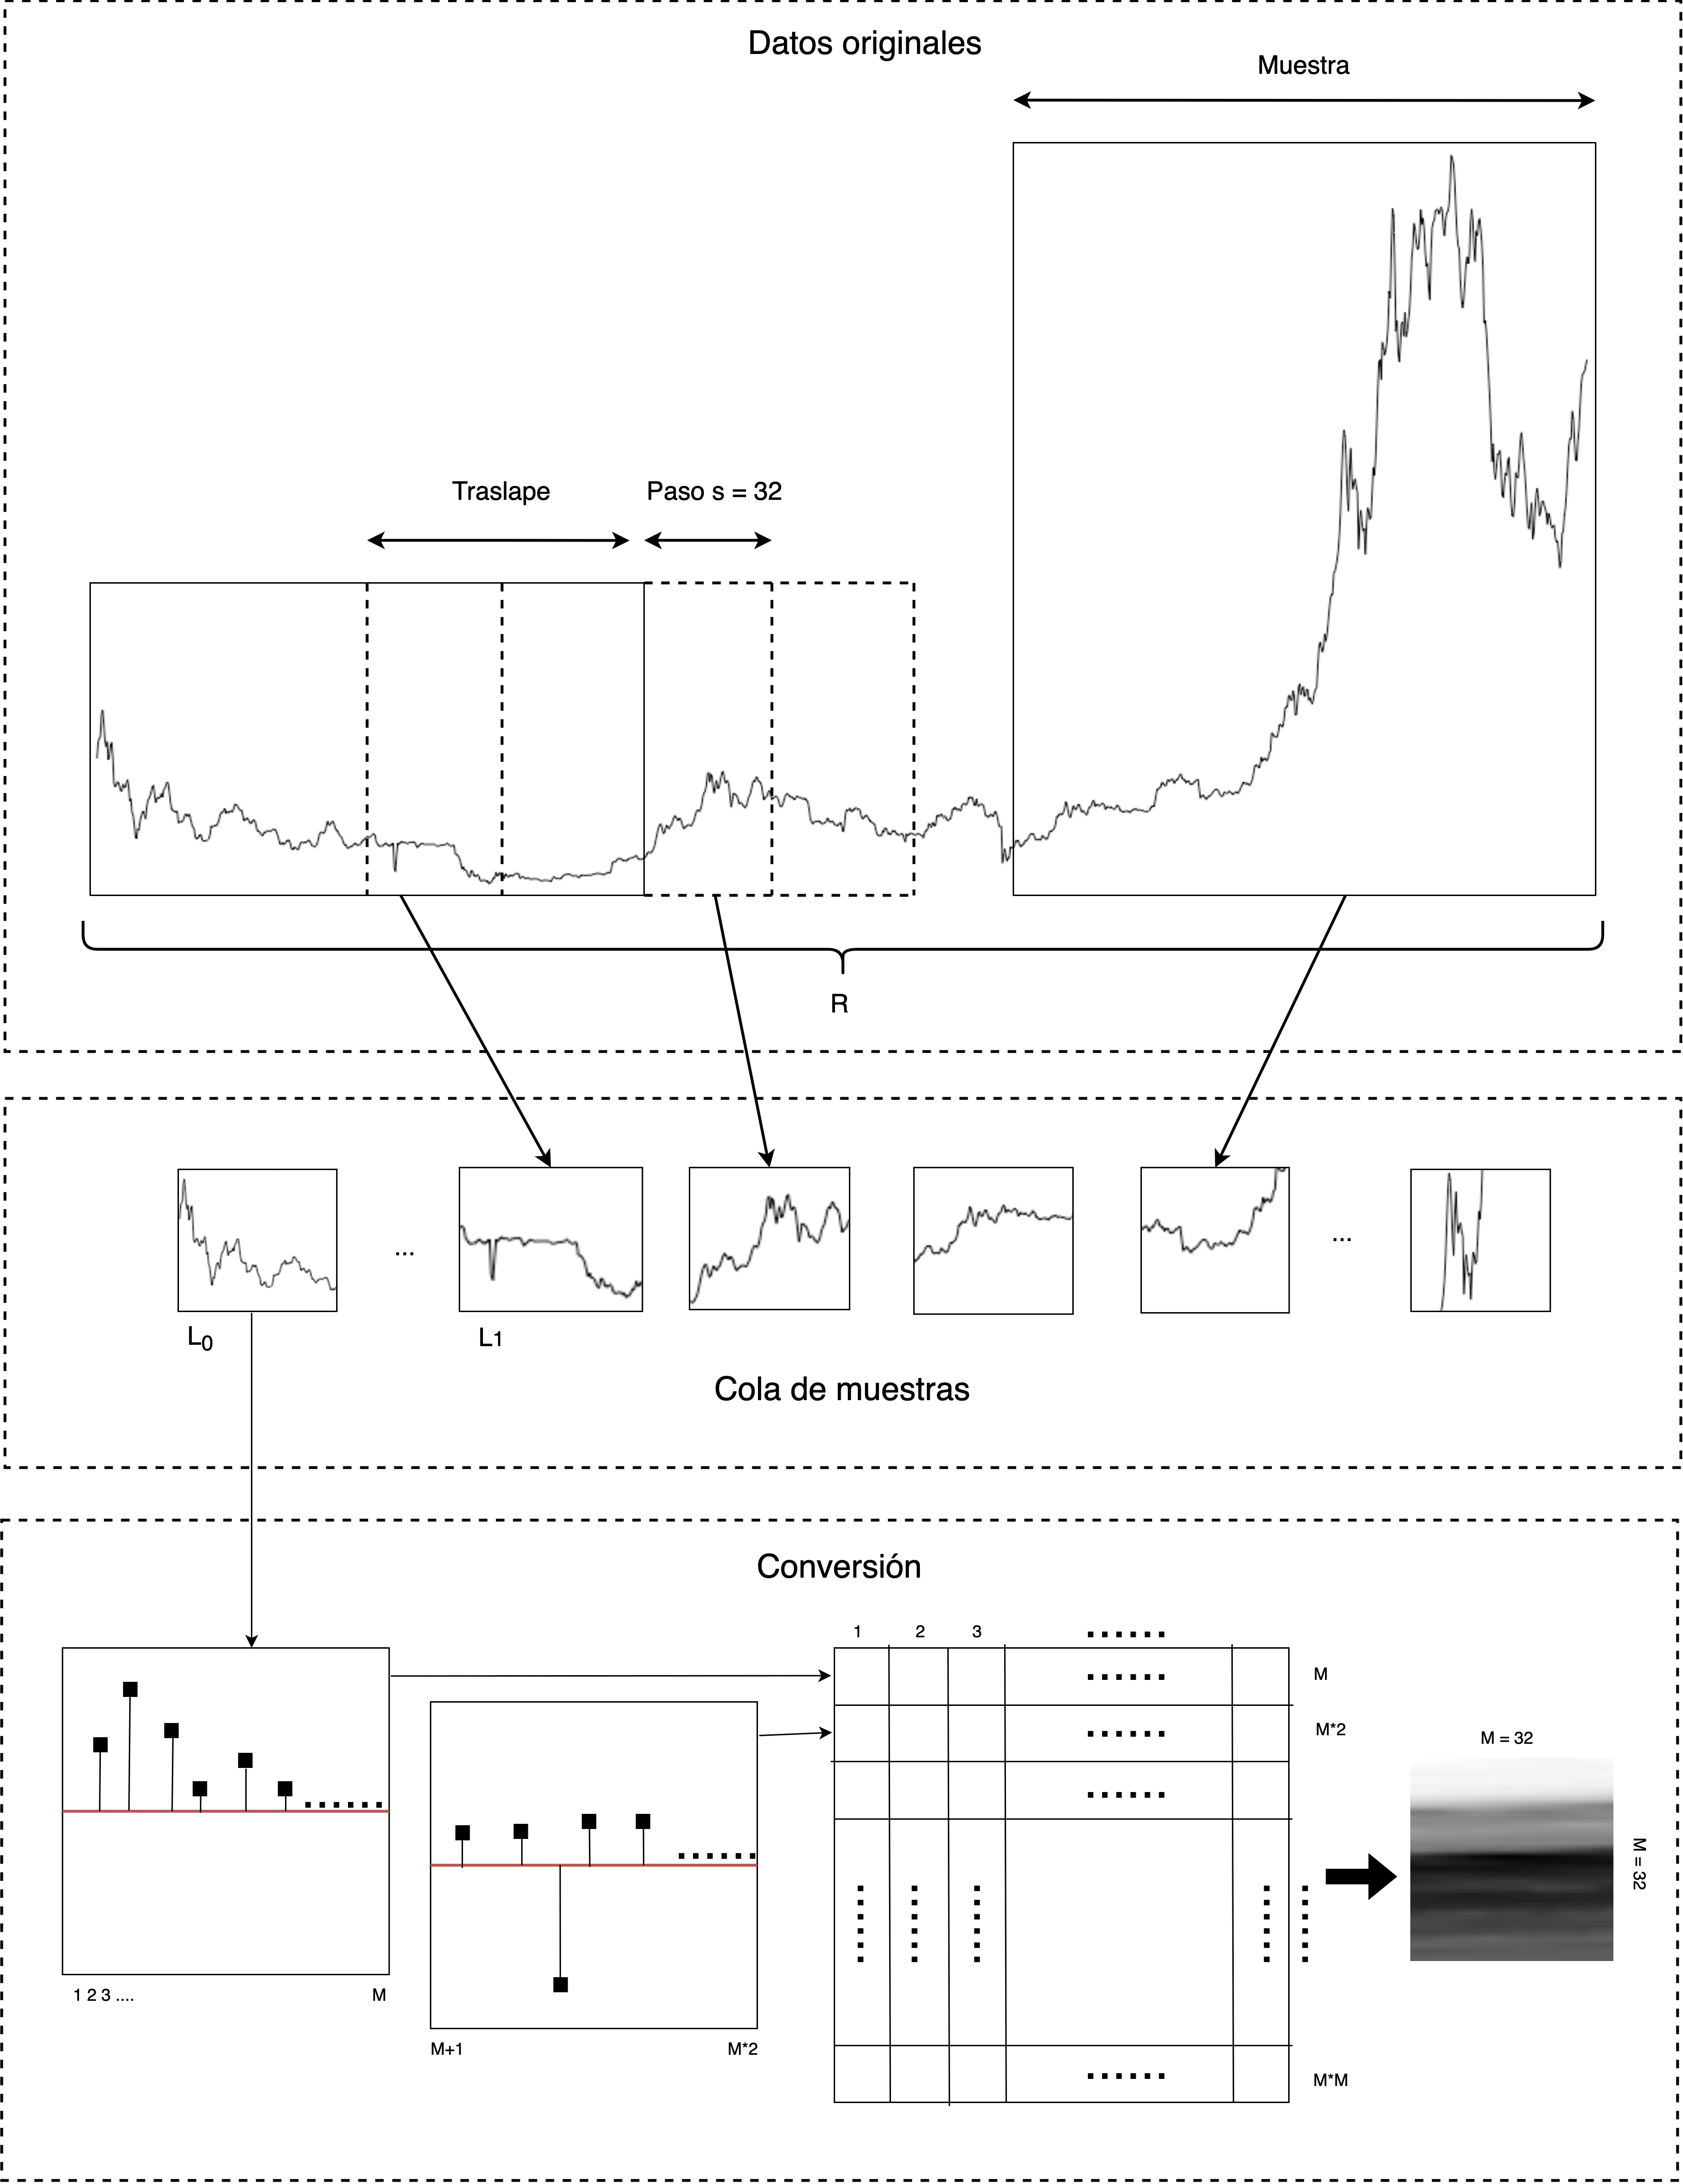
\includegraphics[width=\textwidth,height=21cm]{Chapter3/3-2.png}
	\caption{Método para convertir datos a imágenes.}
	\label{fig: met5}
\end{figure}

\subsection{Selección de métricas}
\label{ssec:metrics}
Para la selección de métricas que más influyen en el precio del bitcoin primero se eliminaron variables con alta multicolinealidad usando el Factor de Inflación de Varianza (VIF) y se seleccionaron aquellas que tuvieran significación estadística usando mínimos cuadrados ordinarios. De las variables seleccionadas se escogieron aquellas que tuvieran la misma dirección y el mismo o mayor peso que la variable $precio$ usando análisis de componentes principales. Al final se corroboró la información usando un dendrograma de correlación para ver la relación entre las variables.

\subparagraph{Factor de Inflación de Varianza (VIF):}

Para realizar el análisis de regresión se evita la multicolinealidad en las variables para obtener resultados con significación estadística verdadera, para ello se usó el método VIF para reducir el conjunto de predictores a un conjunto linealmente independiente. El método utilizado es el siguiente:

\begin{enumerate}
	\item Se seleccionan las variables con una correlación mayor al valor absoluto $0.9$ excluyendo al precio.
	\item Se calcula el VIF del conjunto de variables obtenidos anteriormente.
	\item Se elimina la variable con el VIF más alto y se guarda en una lista.
	\item El proceso se repite hasta que el VIF más alto sea menor que $5$ ya que este representa una correlación moderada.
	\item El conjunto de datos final es el total menos las variables de la lista creada.
\end{enumerate}


\subparagraph{Análisis de regresión:}
\label{AR}
Las variables endógenas utilizadas son las obtenidas en el paso anterior, la variable exógena es el precio en dólares obtenido de Coin Metrics. 
A los datos de entrenamiento de las métricas se ajustó un modelo de mínimos cuadrados ordinarios de la librería statsmodels en Python y se seleccionaron las variables con un valor $p$ menor que $0.05$ con base en el estadístico $t$.

\subparagraph{Análisis de componentes principales:}
\label{PCA}

De las métricas obtenidas utilizando análisis de regresión se seleccionaron aquellas que tuvieran la misma dirección y, mayor o igual magnitud que la variable $precio$, para ello se utilizó la función PCA de la librería \emph{sklearn.decomposition} en Python.
Se utilizó como parámetro la cantidad total de métricas obtenidas anteriormente y se utilizó el siguiente criterio para determinar las métricas con mayor influencia en el precio
\[ \bar{F} = \{ y \hspace{0.5mm}:\hspace{0.5mm} \lVert y \rVert_2 \geq \lVert x \rVert_2,\hspace{0.5mm} \textrm{sign}(y) = \textrm{sign}(x),\hspace{0.5mm}y \in F\}, \]
donde $F$ es el conjunto de características obtenidas en el análisis de regresión, $x$ es el vector de $precio$, $\lVert \cdot \rVert_2$ es la norma euclidiana usual y sign es la función signo.

\subparagraph{Dendrograma de correlación:}
Se utilizó la función heatmap de la librería biokit en Python utilizando todas la características obtenidas en el paso anterior empleando como distancia la correlación entre las métricas y se seleccionaron aquellas que estuvieran en el mismo cluster que el precio o cercanas al mismo.

\subsection{Análisis topológico de datos}
\label{met_tda}
Se siguieron los siguientes pasos para determinar los posibles cracs en el precio:

\subparagraph{Incrustar los datos en un espacio de dimensión superior:} La serie de tiempo del precio del bitcoin es incrustada en un espacio de dimensión 4 usando el teorema de Takens.
\subparagraph{Creación del panorama de persistencia:} Con los datos en un espacio de dimensión superior se calcula la homología persistente de los datos para crear el respectivo panorama de persistencia. Se utiliza la librería $TDA$ de R con la función $ripsDiag()$.
\subparagraph{Cálculo de norma topológica:} A partir del panorama de persistencia creado en R, al ser un elemento vectorial, se calcula la norma $L^1$ y posteriormente la $C^1$ respectiva definida en la \cref{normastopologicas}.

\subparagraph{Creación de clusters:} Se aplica el algoritmo K-means a un dataframe que tiene por columnas el logaritmo del precio del bitcoin y la norma $C^1$ para visualizar los posibles clusters de los datos.
\subparagraph{Selección de cluster de riesgo:} Con base a los siguientes criterios se selecciona el cluster que nos advierte de una posible burbuja, que se identifica como una sucesión de rendimientos positivos que pueden ser interrumpidos por rendimientos negativos cuya magnitud no supera algún nivel de tolerancia preestablecido, y una caída posterior como una sucesión de rendimientos negativos que pueden ser interrumpidos por rendimientos positivos cuya magnitud no supera el nivel de tolerancia preestablecido \parencite{gideaTopologicalRecognitionCritical2020}. 

\begin{enumerate}
	\item La mayoría de los elementos del cluster cumplen que $\lVert x_t \rVert_{C^1} > 0.5$
	\item Las fechas en el cluster deben ser consecutivas.
\end{enumerate}

El riesgo de esto es que aunque la inversión no sea viable, se seguirán sumando personas incrementando el valor del activo hasta hacerlo insostenible, haciendo perder capital al inversor si este compró en el punto álgido de la sucesión de rendimientos positivos.

\subsection{Validación del modelo}
\subparagraph{Predicción del precio:}
En cada modelo se realizo una predicción sobre el 80\% de los datos, en estas predicciones se consideró el indicador de error RMSE (Root Mean Square Error) y la segunda versión del índice de eficiencia Theil’s U \parencite{bliemelTheilForecastAccuracy1973}.
Hubo un total de 49 modelos tomando en cuenta cada transformación propuesta, de estos, el modelo seleccionado en este estudio es el que tiene menor RMSE e índice Theil’s U más cercano a cero. Con el modelo seleccionado se hace la predicción sobre el conjunto de validación como se muestra en la \cref{subResultados}.

\begin{table}[H]
	\centering
	{
		\begin{tabular}{ll}
			\toprule
			\textbf{Indicador} & \textbf{Fórmula}\\
			\midrule
			RMSE			&$\sqrt{\frac{\sum_{i=1}^{n}({\hat{y_{n}}} - y_{n})^{2}}{n}}$\\ 
			Theil’s U 	&$\sqrt{\frac{\sum_{i=1}^{n}({\hat{y_{n}}} - y_{n})^{2}}{\sum_{i=1}^{n}y_{n}^{2}}}$ \\
			
			\bottomrule
			\hline
	\end{tabular}} \quad
	\caption{Fórmulas de los índices RMSE y Theil’s U.}
	\label{tab:Table12}
\end{table}

\subparagraph{Clasificación del precio:}
Se crea un dataframe con las imágenes generadas. Una columna contiene los archivos de imagen y la otra las etiquetas de su cluster respectivo. Los clusters son renombrados a comprar, vender o arriesgar.

Se crea el conjunto de entrenamiento del dataframe creado, se configura la CNN como en la \cref{tab:Table11} y se entrena con los datos anteriores.

La precisión del modelo es calculada utilizando el método accuracy de tensorflow la cual crea dos variables locales, \emph{total} y \emph{count}, que se utilizan para calcular la frecuencia con la que las predicciones coinciden con las etiquetas. Esta frecuencia se devuelve finalmente como una operación que simplemente divide el total entre el recuento.





